\subsection{Einrichten der Projektumgebung}
Für die Entwicklung der \ac{pwa} wird die Entwicklungsumgebung \textit{WebStorm} von JetBrains gewählt, da sie die gehäuften Routineaufgaben selbstständig bzw. mit geringem Aufwand ausführt.

Wie für die Entwicklung der meisten modernen Webanwendungen ist die Installation der \textit{Node.js}-Laufzeitumgebung notwendig. Mit dem integrierten Paketmanager \texttt{npm} lassen sich Bibliotheken leicht zum Projekt hinzufügen.
Um die \textit{Angular}-Anwendung automatisiert zu erstellen, ist zuerst die Installation des \textit{Angular \acl{cli}} \acs{cli} erforderlich. Mit dem Konsolenbefehl \texttt{npm install -g @angular/cli} wird \texttt{npm} aufgefordert, die neuste Version der Angular \ac{cli} global auf dem System zu installieren.

Mit dem Befehl \texttt{ng new todoapp} wird die Angular \ac{cli} (in der Konsole als \texttt{ng} abgekürzt) dazu gebracht, ein Angular-Projekt inklusive nötiger Dateistrukturen zu erstellen.

\begin{figure}[h!]
	\centering
	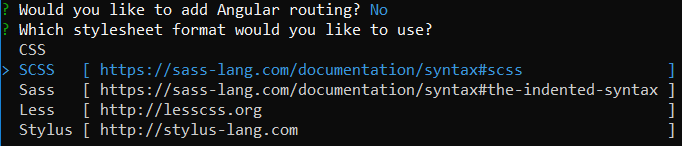
\includegraphics[width=0.58\textwidth]{img/angular_cli_css.PNG}
	\caption{Stylesheet-Formate beim Erstellen der Angular-Anwendung}
	\label{fig:stylesheet_formate_cli}
\end{figure}

Die \ac{cli} bietet dem Nutzer einige Optionen bei der Erstellung an, die jedoch in diesem Projekt nicht zwangsläufig benötigt werden. So kann bspw. ein Routing oder Unit-Testing eingerichtet werden.
Außerdem unterstützt die \ac{cli} verschiedene Stylesheet-Formate (siehe Abb. \ref{fig:stylesheet_formate_cli}). Das ist für Entwickler sehr praktisch, wenn sie einen dieser \ac{css}-Dialekte beherrschen. Die Arbeit mit Variablen in Stylesheets bevorzugt wird, werden in diesem Projekt \acsu{scss}-Dateien verwendet

\subsection{Aufbau der Anwendung mit Angular}

Im Folgenden werden die einzelnen Komponenten der \textit{Angular}-Anwendung erläutert.
\subsubsection{Bereitstellen der Klasse \texttt{TodoItem} zur Datenspeicherung}

Die Komponenten tauschen untereinander Daten aus. Damit diese einer einheitlichen Struktur folgen, wird eine Klasse \texttt{TodoItem} erstellt, die einen To-Do-Eintrag repräsentiert. Objekte dieser Klasse können nun zwischen Komponenten ausgetauscht und modifiziert werden.

\begin{listing}[h!]
	\inputminted{TypeScript}{sourcecode/pwa_todoitem_klasse.js}
	\vspace{-0.5cm}
	\caption{\texttt{TodoItem}-Klasse zur Datenspeicherung (TypeScript)}
	\label{sourcecode:todoitem_klasse}
\end{listing}
\vspace{-0.5cm}

Wie im Quellcode-Ausschnitt \ref{sourcecode:todoitem_klasse} zu sehen, hat ein To-Do-Element eine Aufgabenbeschreibung (Z. 2), eine eindeutige ID (Z. 3) sowie zwei boole'sche Werte, die speichern, ob das Element als priorisiert oder abgeschlossen markiert worden ist (Zz. 4--5). Die ID hilft später, ein bestimmtes To-Do-Element zu modifizieren.

\subsubsection{Implementierung des \texttt{todoService} für die Datenverwaltung}
Alle To-Do-Einträge sollen persistent auf dem Gerät gespeichert werden. Dafür wird ein Angular-Service erstellt; der \texttt{todoService}. Er ist für die \ac{crud}-Operationen zuständig.

\begin{listing}[h!]
	\inputminted{TypeScript}{sourcecode/pwa_todo_service.ts}
	\vspace{-0.5cm}
	\caption{Klasse \texttt{TodoService} (TypeScript)}
	\label{sourcecode:pwa_todo_service}
\end{listing}
\vspace{-0.5cm}

In Quellcode-Ausschnitt \ref{sourcecode:pwa_todo_service} sind die Kernfunktionen des Services abgebildet. Der Service speichert ein Array von \texttt{TodoItem}-Objekten. Wenn der Nutzer ein Element hinzufügt, erstellt der Service ein neues Datenobjekt und speichert dieses im Array und dem Browserspeicher (Zz. 16-18). Die Funktionsweise der übrigen \ac{crud}-Operationen ist analog dazu.

Mit \texttt{localStorage} (Zz. 8-14) kann auf den \textit{Key-Value-Store} des Browsers zugegriffen werden. Beim Speichern werden die To-Do-Elemente als \ac{json}-Objekt im Store abgelegt und analog dazu geladen. Der Key-Value-Store verliert seine Daten beim Schließen der Seite nicht und besitzt kein Ablaufdatum, wie bspw. ein Cookie \cite{LocalStorage}.

\begin{figure}[h!]
	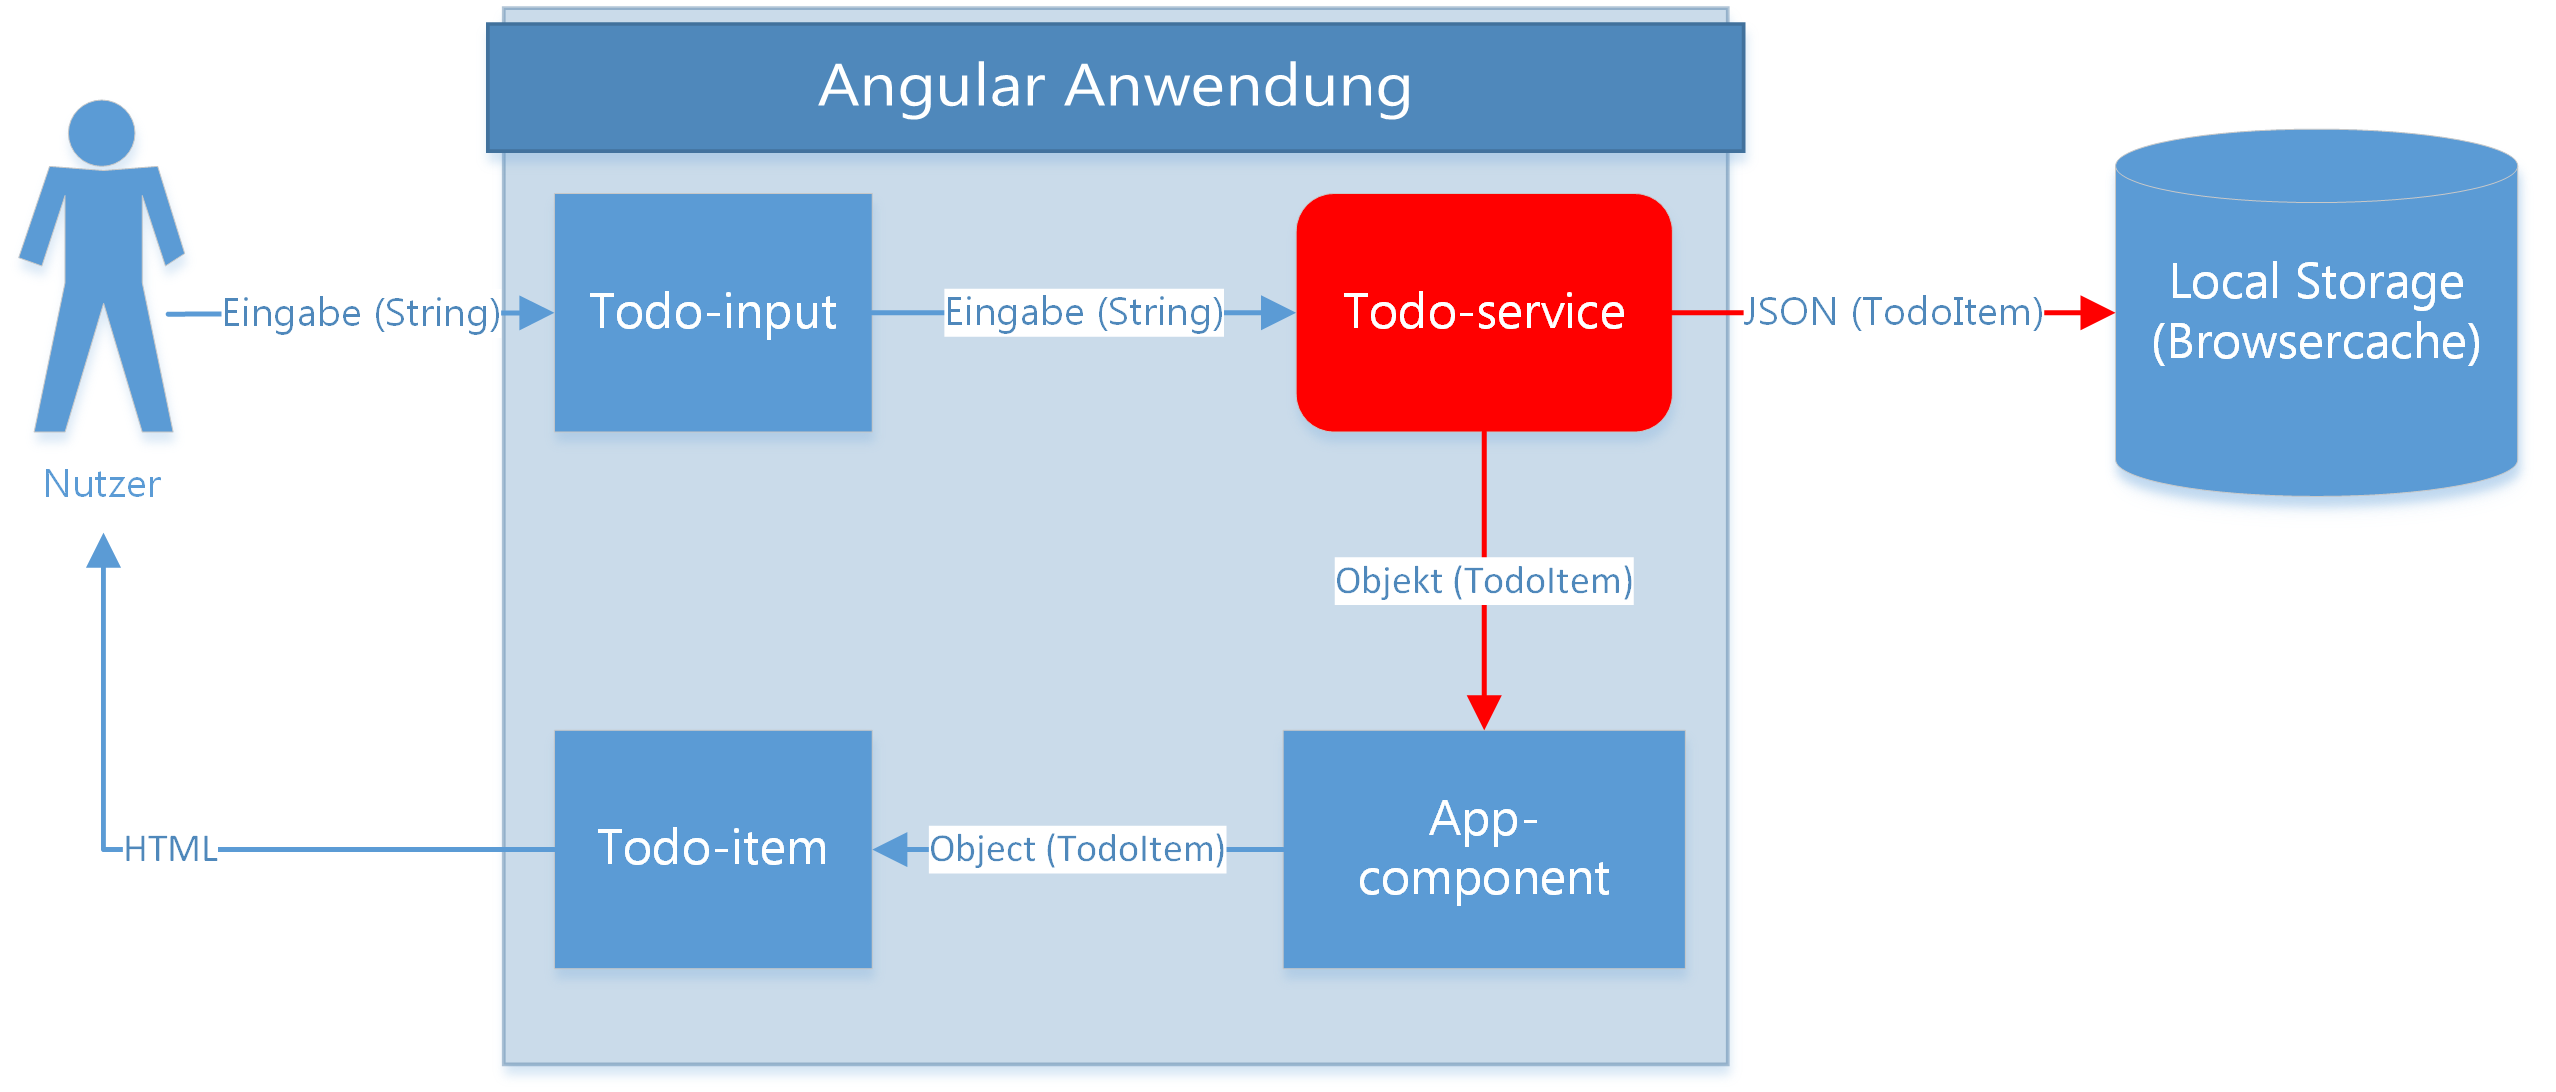
\includegraphics[width=\textwidth]{img/pwa_datenfluss_erstellen.png}
	\centering
	\caption{Datenfluss bei Erstellung eines To-Do-Eintrages}
	\label{fig:pwa_datenfluss_erstellen}
\end{figure}

Abb. \ref{fig:pwa_datenfluss_erstellen} zeigt den Datenfluss beim Erstellen eines To-Do-Eintrags. Die To-Do-Beschreibung wird vom Nutzer über ein Eingabefeld an den Service weitergereicht. Dieser erstellt ein entsprechendes Datenobjekt und reicht es an die Stammkomponente weiter, worüber schlussendlich \ac{html}-Code erzeugt werden kann. Gleichzeitig speichert er das neue Element im Browserspeicher ab.

\subsubsection{Beschreibung der Dateistruktur und Komponenten der Angular-Anwendung}
Nach dem im Vorangegangenen beschrieben worden ist, wie das Projekt erstellt worden ist, wird im Folgenden detaillierter auf das erstellte Angular-Projekt eingegangen. Angular, welches stark komponentenorientiert aufgebaut ist, zeigt sich auch in seiner Dateistruktur stark komponentenbezogen. In Abb. \ref{fig:pwa_dateistruktur} sind die wichtigsten Dateien in einem Diagramm dargestellt.

\begin{figure}[h!]
	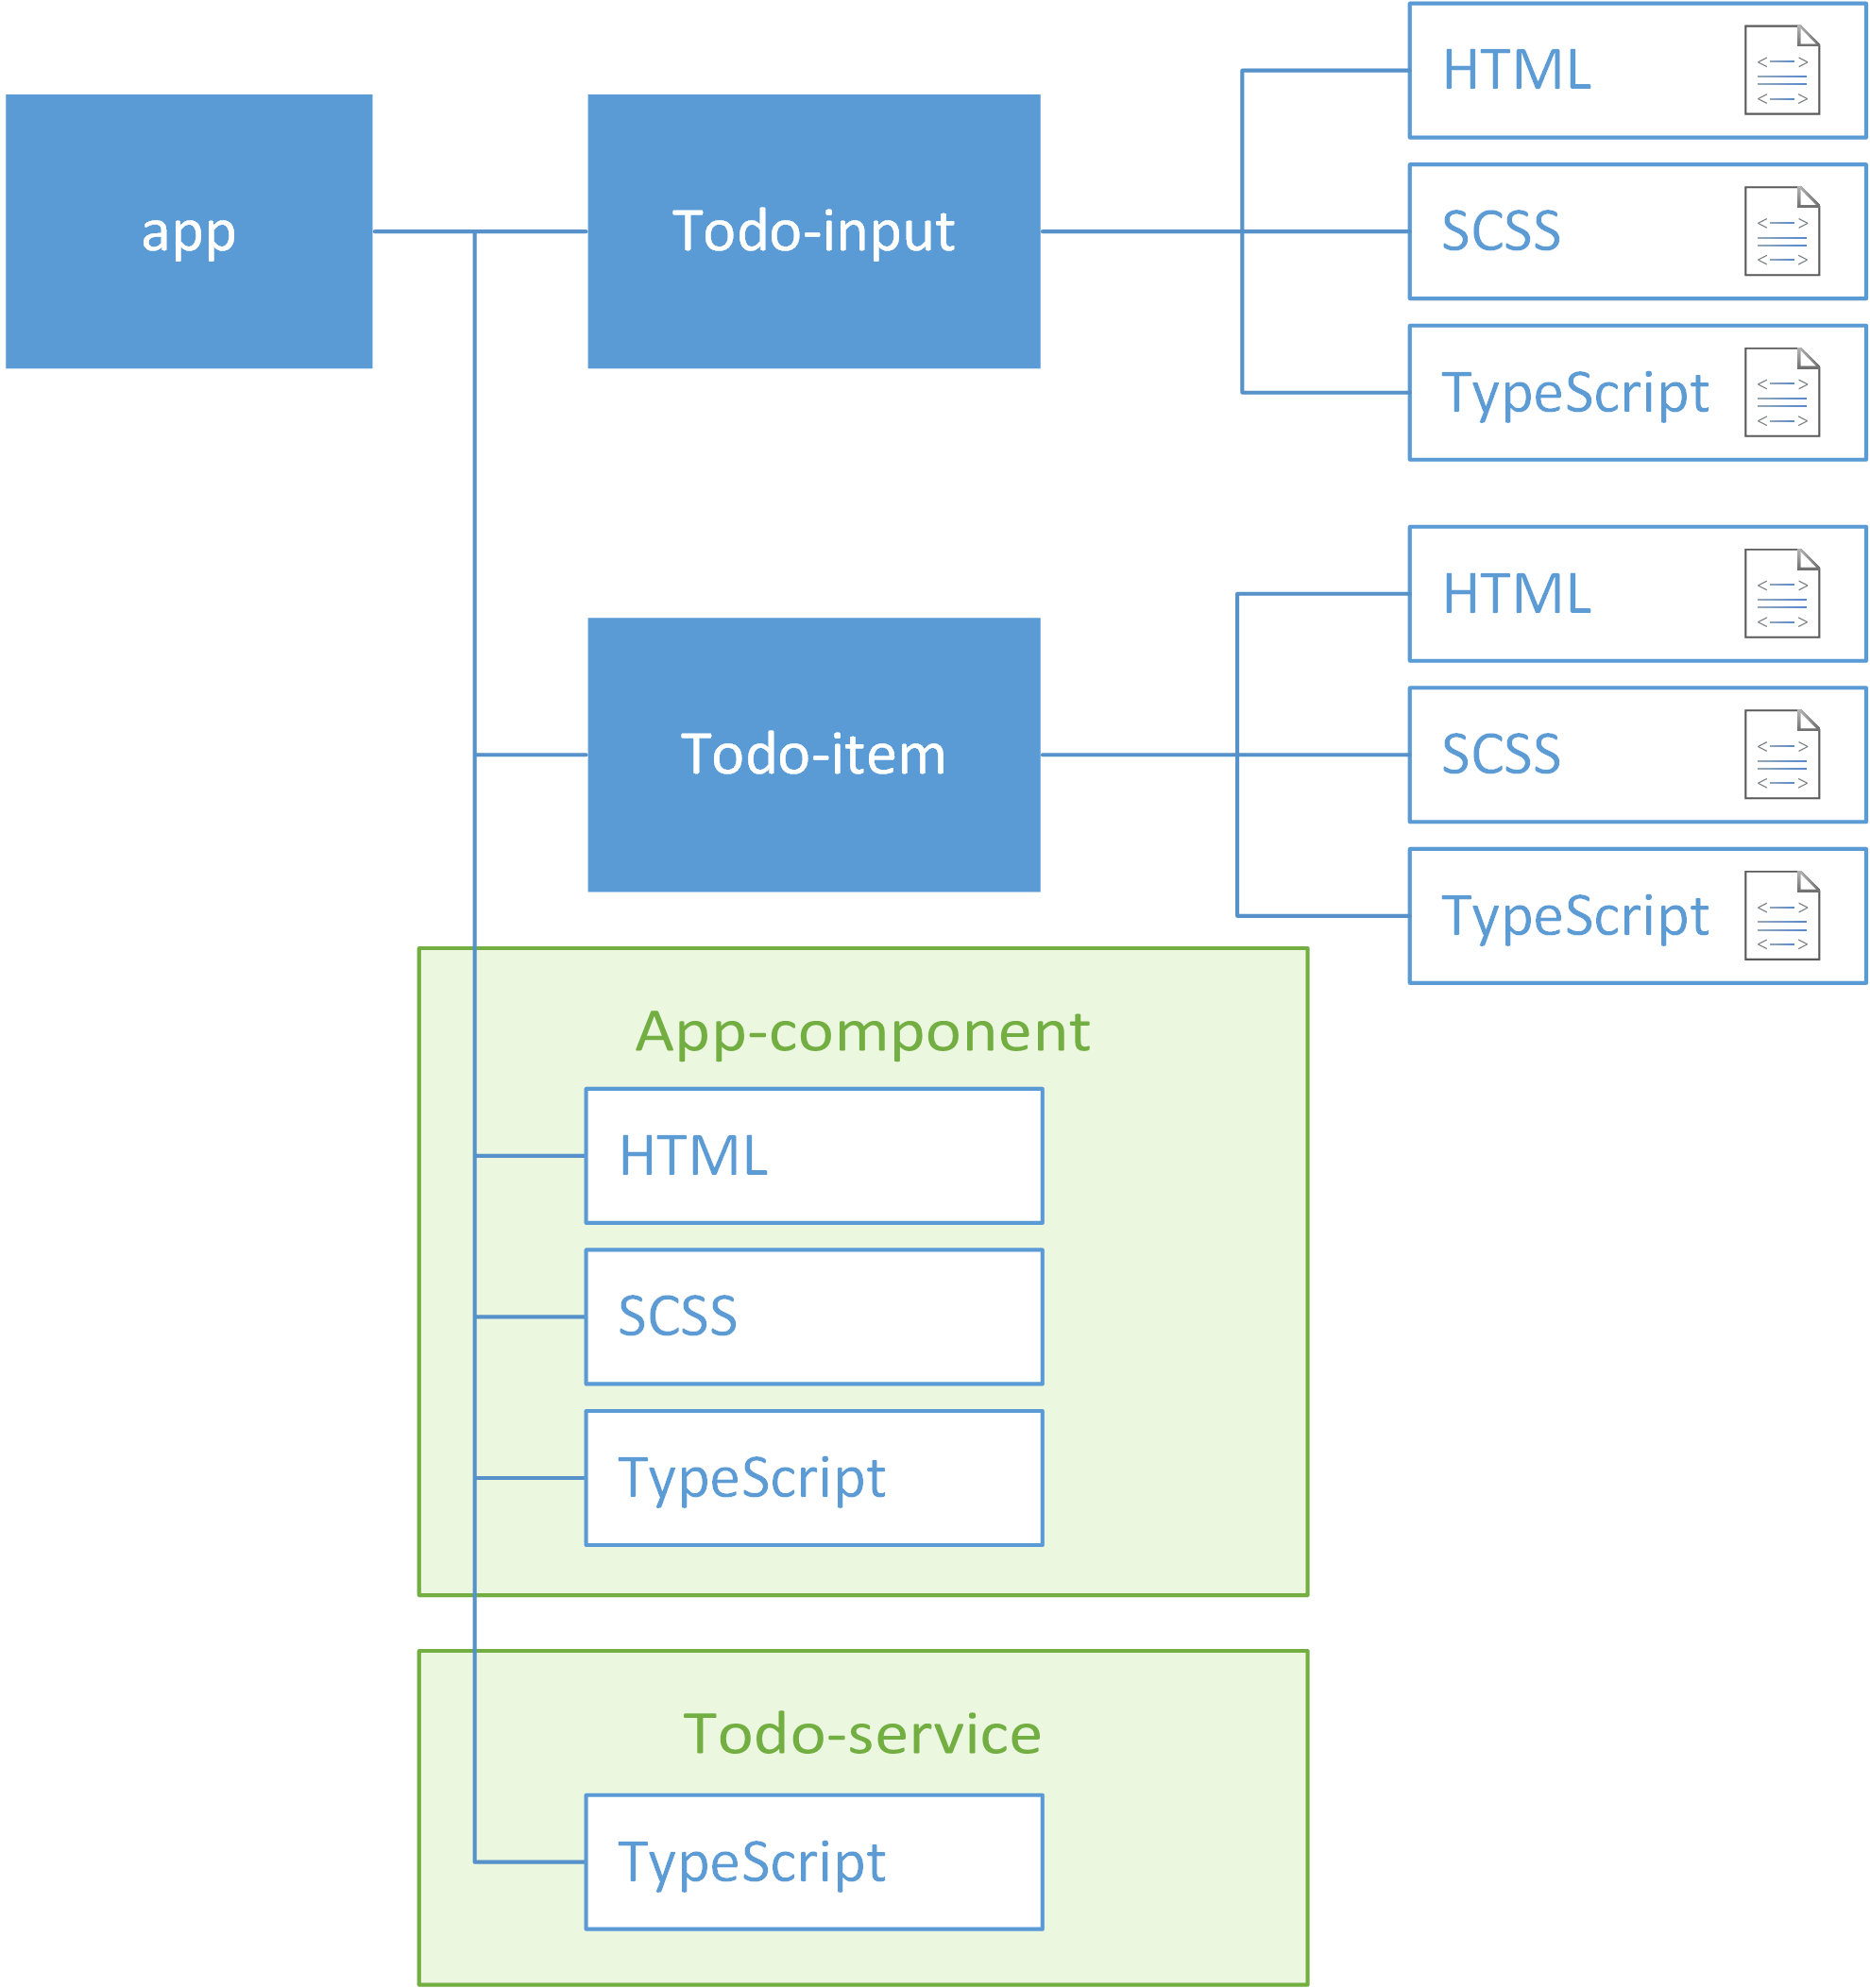
\includegraphics[width=0.6\textwidth]{img/pwa_dateistruktur.png}
	\centering
	\caption{Datei-Struktur der Angular-Anwendung}
	\label{fig:pwa_dateistruktur}
\end{figure}

\begin{description}
	\item[Stammkomponente] Zunächst befinden sich im \texttt{app}-Verzeichnis eine \ac{html}-, eine Stylesheet- und eine TypeScript-Datei des \texttt{app-component}, welcher die Stammkomponente darstellt. Sie dient als Container (Begriffserklärung s. Sektion \ref{sec:2-1_begriffsdefinitionen}) um die To-Do-Elemente und das Eingabefeld (siehe Ausschnitt \ref{sourcecode:pwa_app_component_html}, Z. 5).
	
	\begin{minipage}{\linewidth}
		\inputminted{ng2}{sourcecode/pwa_app_component.html}
		\vspace{-0.5cm}
		\captionof{listing}{\acs{html}-Template des \texttt{app-component} (Angular \acs{html})}
		\label{sourcecode:pwa_app_component_html}
	\end{minipage}
	
	\vspace{0.5cm}
	Quellcode-Ausschnitt \ref{sourcecode:pwa_app_component_html} (Zz. 1--3), zeigt, wie die Daten aus dem \texttt{todoService} in \ac{html}-Code dargestellt werden. Wie in einer \texttt{for}-Schleife wird jedes item des \texttt{todoService} einer neu erstellten \texttt{todo-item}-Komponente übergeben.
	Angular wird das \ac{html}-Template automatisch neu rendern, wenn sich die Elemente im \texttt{todoService} ändern.	
	
	\item[To-Do-Element] 
	Das \texttt{todo-item} ist ein einzelnes Elemente der To-Do-Liste. Es enthält einen Button zum priorisieren, eine Checkbox zum Abhaken des Elements, eine Textbox und einen Button zum Löschen (s. Abb. \ref{fig:pwa_todo_item_screenshot}).
	\newpage
	\begin{minipage}{\linewidth}
		
\includegraphics[width=0.6\textwidth]{img/pwa_todo_item.PNG}
		\centering
		\captionof{figure}{Gerenderte \texttt{todo-item}-Komponente}
		\label{fig:pwa_todo_item_screenshot}
	\end{minipage}
	
	\vspace{0.5cm}
	Es ist sinnvoll, jedes Listenelement in einer mehrfach instanziierten Komponente zu repräsentieren. Dies kapselt die Daten des Listenelements und die Kommunikation mit dem \texttt{todoService} von anderen Listenelementen ab. Wie bereits erwähnt, bekommt jede \texttt{todo-item}-Komponente genau ein Objekt der Klasse \texttt{TodoItem} übergeben.
	
	\begin{minipage}{\linewidth}
		\inputminted{ng2}{sourcecode/pwa_todo_item.html}
		\vspace{-0.5cm}
		\captionof{listing}{\acs{html}-Template des \texttt{todo-item} (Angular \acs{html})}
		\label{sourcecode:pwa_todo_item_html}
	\end{minipage}
	
	\vspace{0.5cm}
	Quellcode-Ausschnitt \ref{sourcecode:pwa_todo_item_html} zeigt das \ac{html}-Template des \texttt{todo-item}s. Die ersten drei Input-Elemente werden durch \texttt{[(ngModel)]} mit einer \textit{Property} (dt. \textit{Eigenschaft}) des \texttt{TodoItem}s verknüpft, welche in der \texttt{todo-item}-Komponente gespeichert wird. Dies bewirkt folgenden Mechanismus: Wird das Input-Element verändert, ändert sich auch das gespeicherte \texttt{TodoItem}. Wird das \texttt{TodoItem} im Code modifiziert, aktualisiert sich das Input-Element entsprechend.
	
	Um modifizierte Daten auch in der Datenquelle zu speichern, wird das modifizierte \texttt{TodoItem} bei jeder Änderung dem \texttt{todoService} übergeben.
	
\end{description}

\subsubsection{Kommunikation der Komponenten mit dem \texttt{todoService}}

Abb. \ref{fig:pwa_todo_service} fasst die Architektur der Angular-Anwendung zusammen. Den zentralen Punkt der Anwendung bildet der \texttt{TodoService}. \newpage
\begin{figure}[h!]
	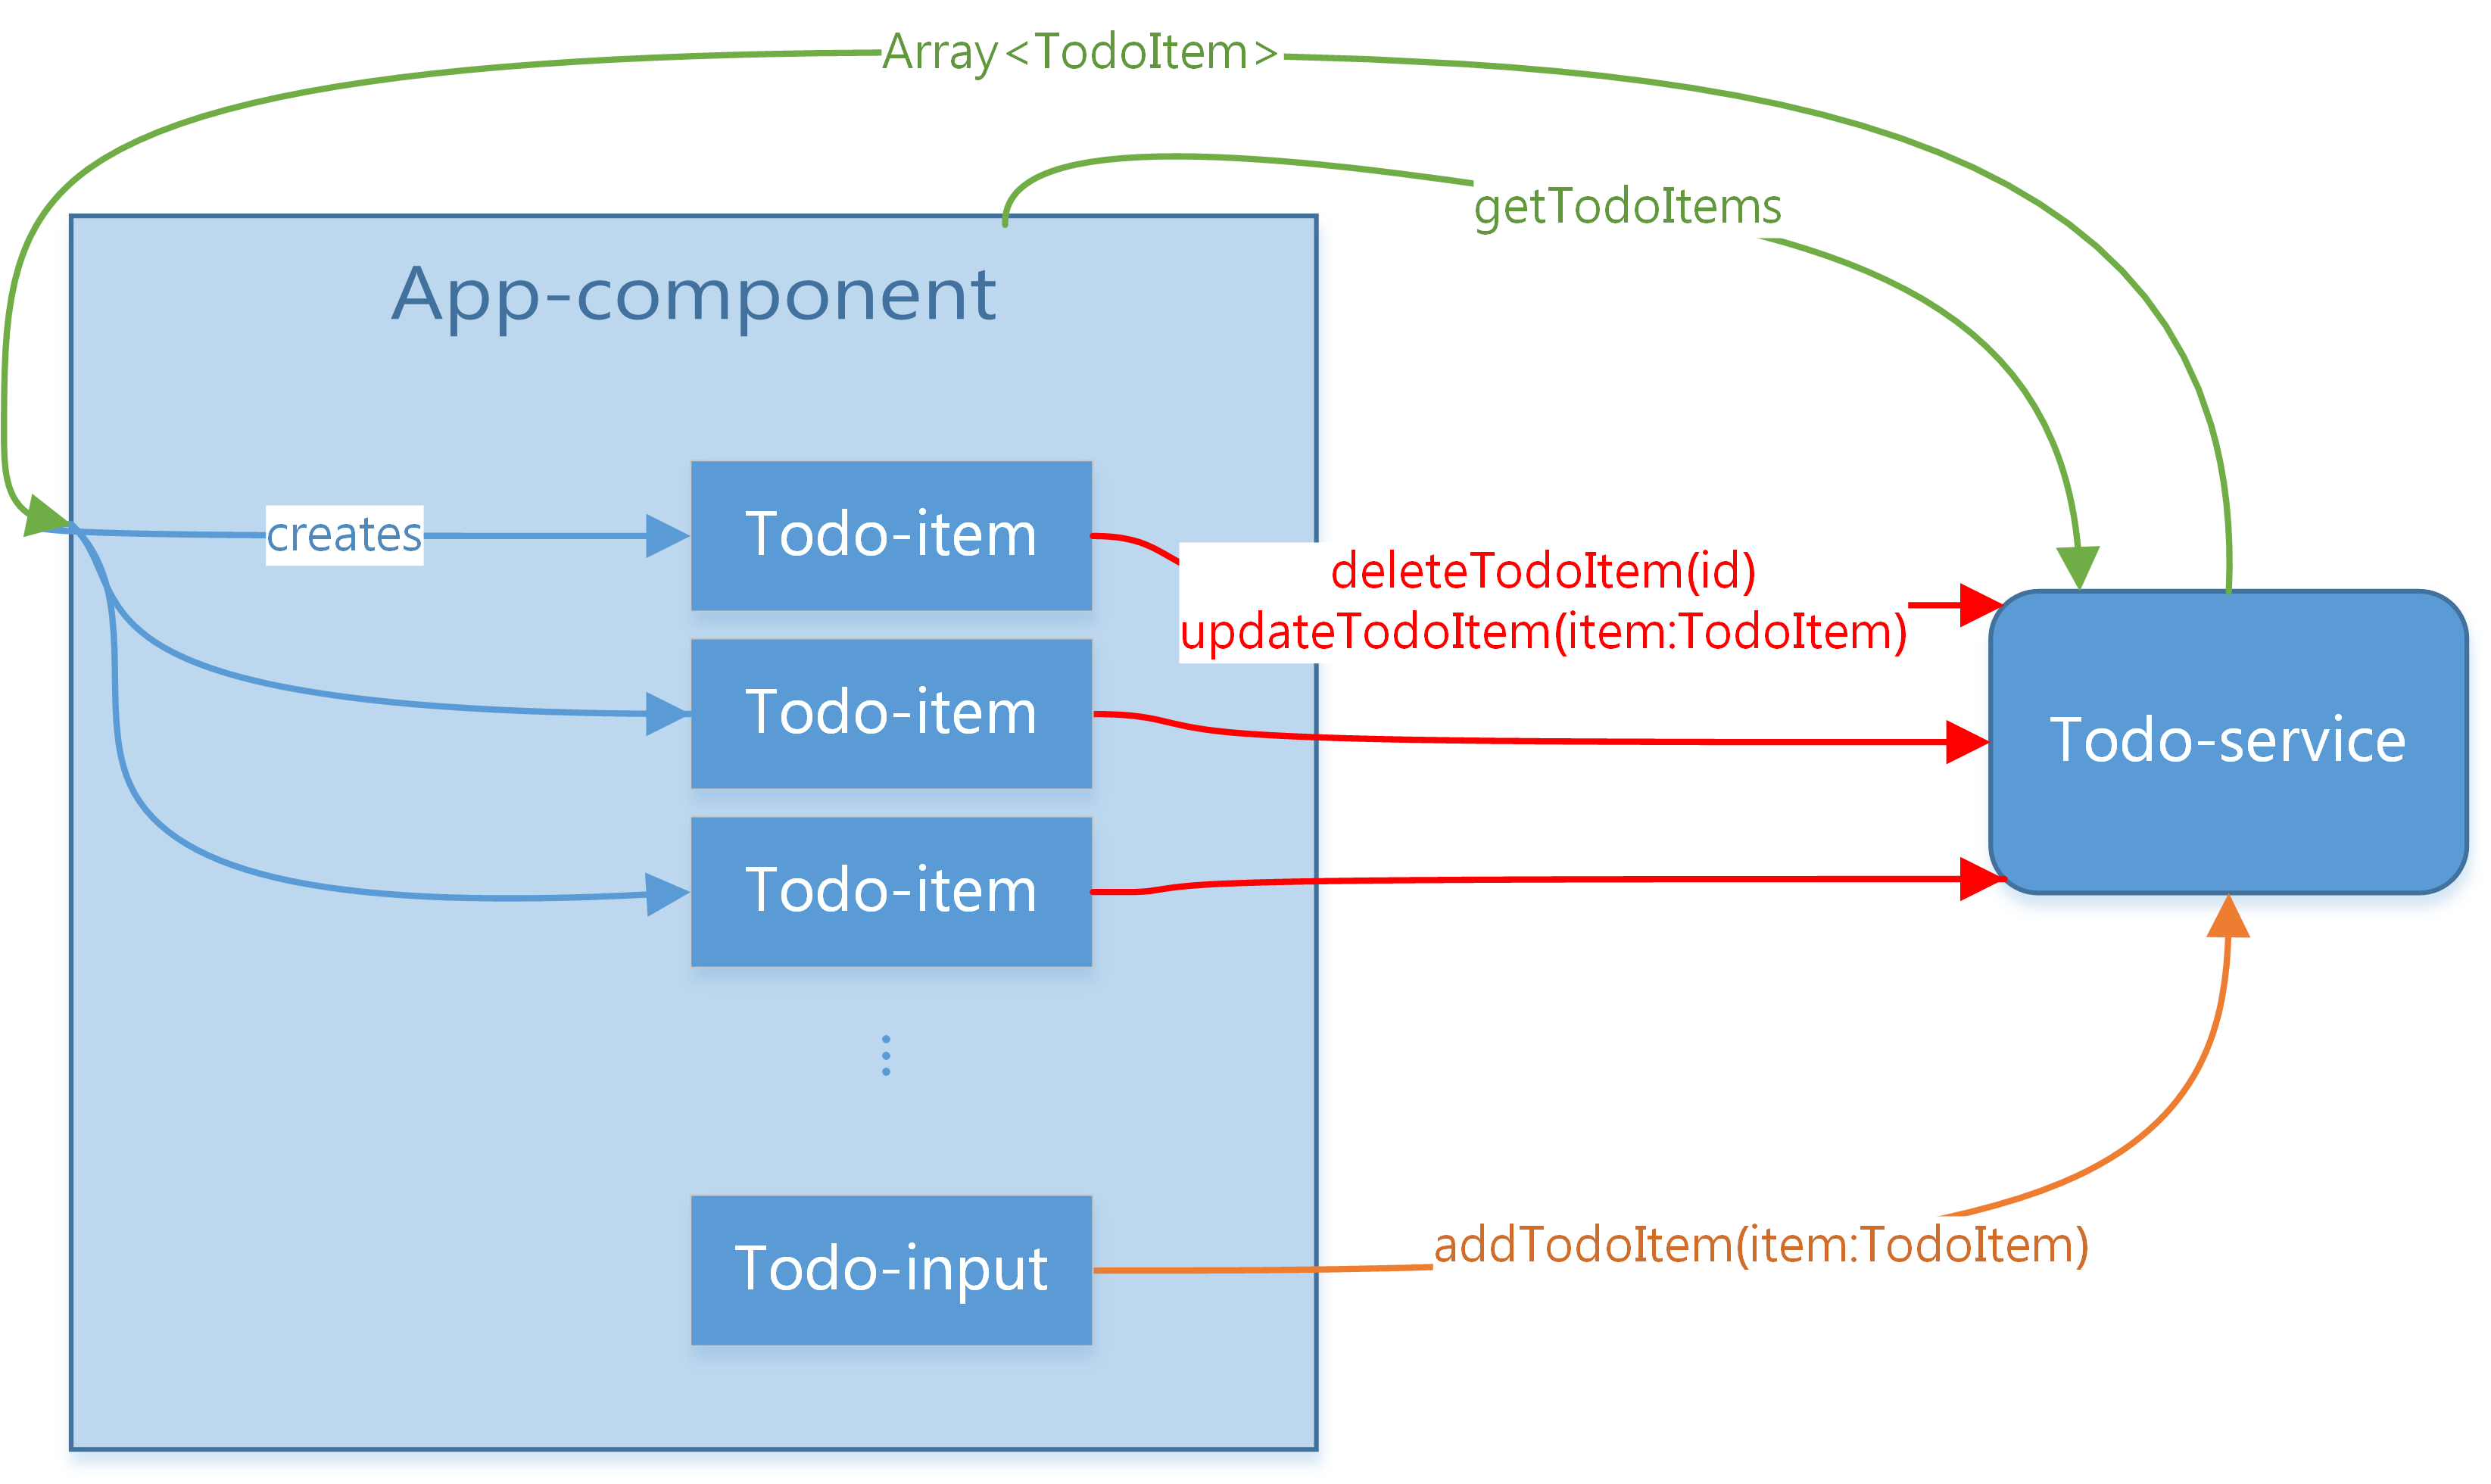
\includegraphics[width=\textwidth]{img/pwa_components.png}
	\centering
	\caption{Interaktion des \texttt{todoService} mit den Komponenten}
	\label{fig:pwa_todo_service}
\end{figure}



Grün dargestellt ist der Datenfluss der gespeicherten To-Do-Elemente zwischen der Stammkomponente und dem \texttt{todoService}. Die Stammkomponente erhält ein Array aus \texttt{TodoItem}s und wird von Angular automatisch aktualisiert, wenn dieses sich ändert.
Die Stammkomponente erstellt für jedes \texttt{TodoItem} eine \texttt{TodoItem}-Komponente (blau dargestellt), die so als Listeneintrag sichtbar wird.

Orange dargestellt ist das Einfügen von Daten durch den Nutzer im Input-Feld der App. Der Input stellt dem \texttt{todoService} ein neues \texttt{TodoItem}-Objekt bereit.

Rot dargestellt ist das Löschen oder Aktualisieren von Items. Wird der Button zum Entfernen gedrückt, oder ändert sich das gespeicherte \texttt{TodoItem}-Objekt der \texttt{TodoItem}-Komponente, werden die Änderungen dem \texttt{todoService} weitergegeben.
Für das Löschen reicht allerdings die einzigartige ID des Objekts aus.

\subsubsection{Gestaltung des \acl{ui}}
Das Styling des von Angular erzeugten \ac{html}-Codes erfolgt mittels \ac{css}. In den bereits erwähnten \ac{css}-Dateien wird den einzelnen Elementen ein Style hinzugefügt.
Erwähnenswert ist dabei, dass alle Anforderungen im Code einzeln beschrieben werden müssen, d.h. Schriftart, Position, Farbe, etc. sind einzeln zu deklarieren.

Mit der Nutzung der \ac{css}-Eigenschaft \textit{Flexbox} lassen sich Elemente responsiv gestalten. Die Nutzung eines \ac{css} oder \ac{ui}-Frameworks würde diese Aufgabe in einem größeren Projekt erleichtern. Mit bekannten Frameworks, wie bspw. dem \textit{Material \ac{ui}}-Framework von Google, lassen sich Elemente dem Material-Design-Prinzip anpassen (vgl. \cite{MaterialUI}), dass auf ähnliche Weise auch bei Android genutzt wird. Hierzu existieren eine Vielzahl von Frameworks mit eigenen Designphilosophien, auf die in dieser Arbeit nicht weiter eingegangen wird.

\begin{figure}[h!]
	\centering
	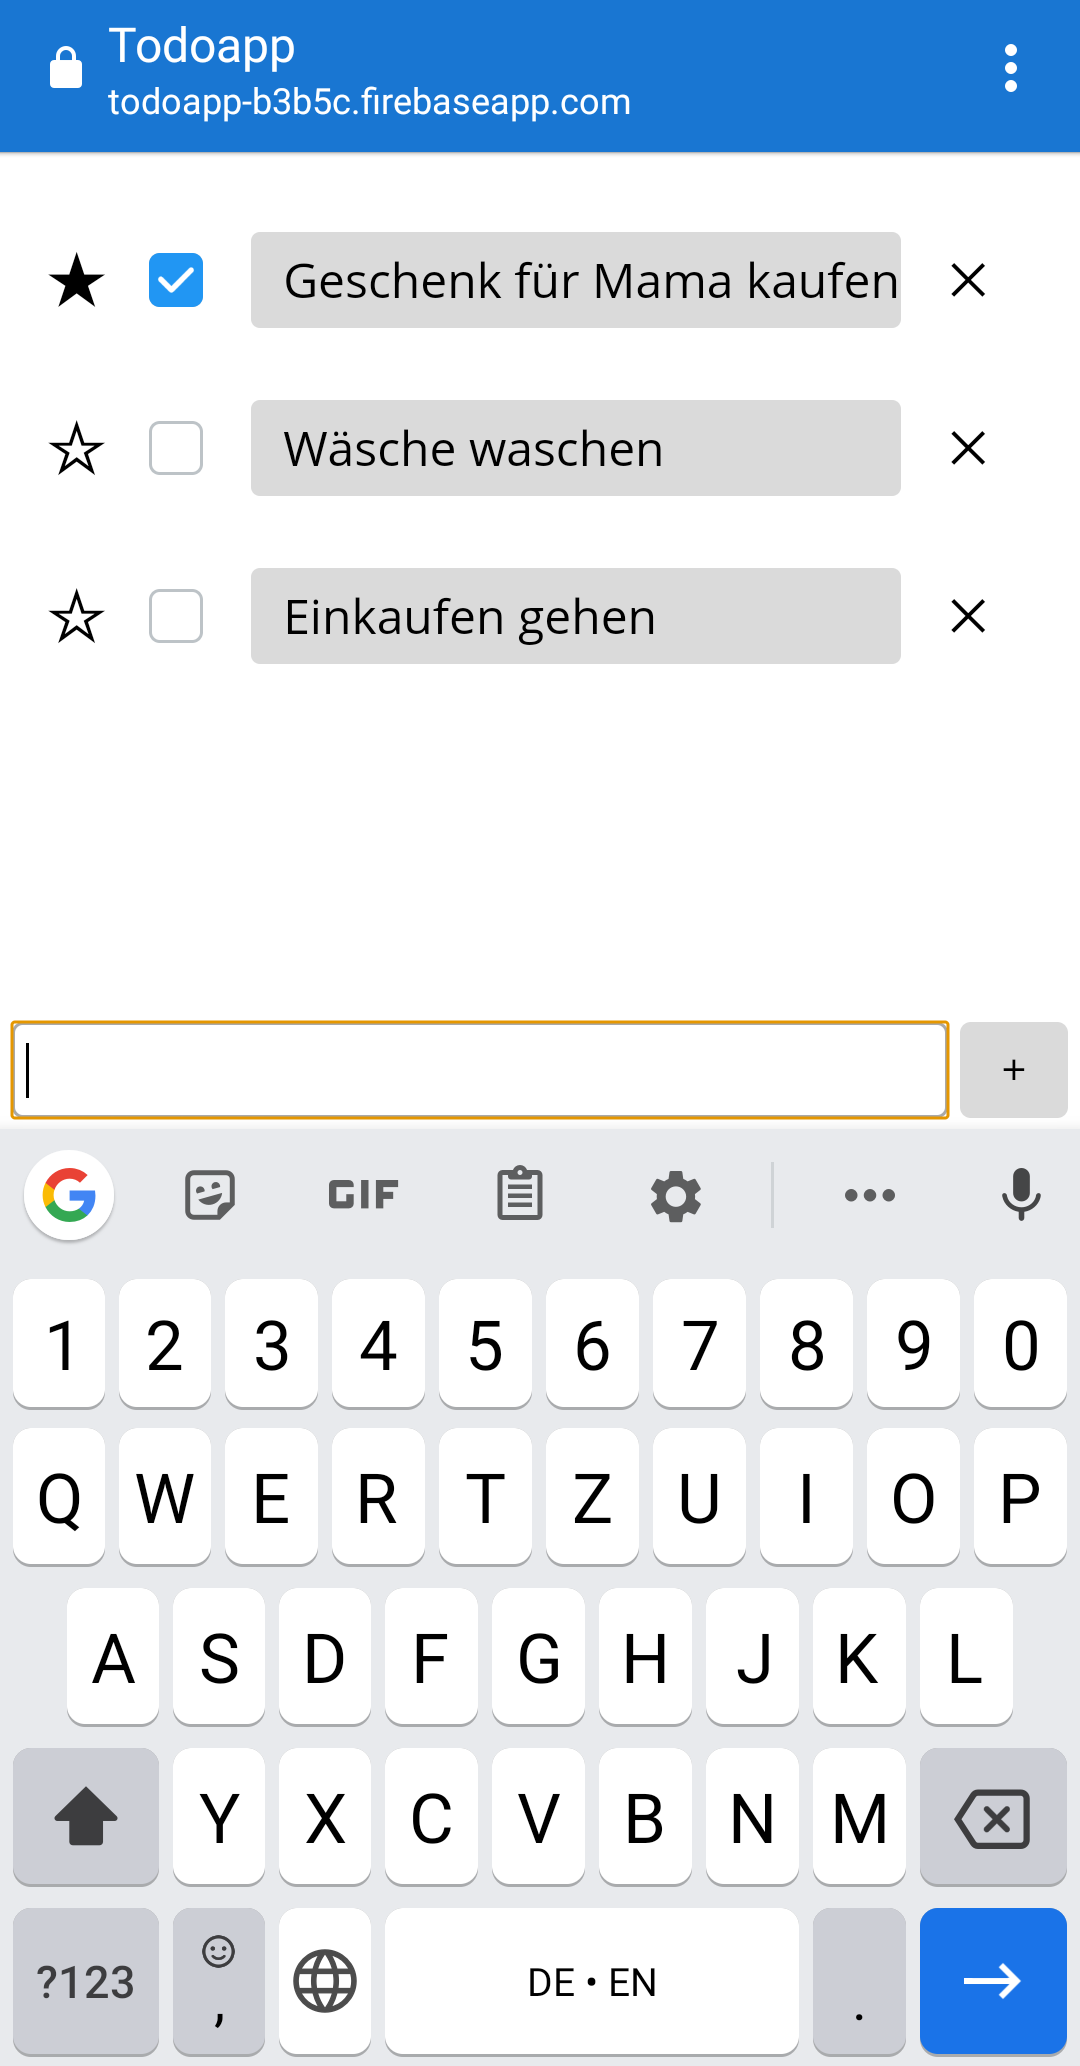
\includegraphics[width=0.38\textwidth]{img/pwa_screenshot_mit_tastatur.png}
	\caption{Screenshot der \ac{pwa} mit geöffneter Tastatur}
	\label{fig:pwa_mit_tastatur}
\end{figure}

Abb. \ref{fig:pwa_mit_tastatur} zeigt einen Screenshot der \ac{pwa}, nachdem diese auf dem Gerät installiert wurde. Tippt der Nutzer in das Eingabefeld, öffnet sich die Tastatur und das \ac{ui} passt sich an die neuen Größenverhältnisse an.

\subsubsection{Umsetzung der Benachrichtigung über unerledigte Aufgaben}
Die definierten Anforderungen geben an, dass der Nutzer an seine Aufgaben erinnert werden soll. In der Praxis stellt sich jedoch heraus, dass die Web-Push-Benachrichtigungen über den Browser zwar sehr gut mit Webanwendungen funktionieren, aber nicht mit \ac{pwa}s ohne Internetverbindung. Mit einem Server, der zu einem bestimmten Zeitpunkt eine Nachricht an die Webanwendung schickt, ist die Umsetzung möglich, allerdings nur bei bestehender Internetverbindung. Die Anforderung wird deshalb als \textit{nicht umsetzbar} betrachtet, da das Kriterium der Offline-Verfügbarkeit nicht umgesetzt werden kann.


\subsection{Integration einer Manifestdatei}

Die Anwendung funktioniert zwar bereits im Browser, ist bislang aber noch keine \ac{pwa}. Um dem Projekt ein \textit{Manifest} und einen \textit{Service Worker} hinzuzufügen, kann wieder das Angular \ac{cli} verwendet werden. \texttt{ng add @angular/pwa} erzeugt die entsprechenden Dateien automatisch, fügt eine \texttt{manifest.json}-Datei hinzu und bindet diese in die \texttt{index.html}-Datei des Projekts ein.

Es ist festzuhalten, dass das Hinzufügen der \ac{pwa}-Funktionalität keinen nennenswerten Aufwand mit sich bringt, wenn das Ziel ausschließlich die Installation der Web-App ist.

\subsection{Hosting der App mit Firebase}
Damit die \ac{pwa} als solche installiert werden kann, muss sie bestimmte Kriterien erfüllen (s. Sektion \ref{sec:2-4_pwa}). Darunter ist die Notwendigkeit der Bereitstellung über \ac{https}. Dies gestaltet sich in der Praxis schwierig, da der Angular-Entwicklungsserver zwar auf \ac{https} konfiguriert werden kann, jedoch selbst signierte \acsu{ssl}-Zertifikate nicht akzeptiert werden. Die \ac{pwa} kann somit nicht installiert werden. Für die Entwicklung ist dies natürlich problematisch, sodass eine Lösung für dieses Problem gefunden werden muss.

Für die spätere Evaluation ist der hier verwendete Hosting-Anbieter nicht relevant. Es gibt zahlreiche Alternativen, die den Anforderungen an das Hosting der Anwendung gerecht werden. Auf diese soll hier aber nicht weiter eingegangen werden. Da das Projekt jedoch aus angeführten Gründen gehostet werden muss, wird das Hosting stellvertretend mit einem Google-Service erläutert.

Googles stellt eine schnelle und elegante Lösung zum Hosten einer Webanwendung bereit: \textit{Firebase}. Über die \textit{Firebase Console}, eine Webanwendung zur Verwaltung von Firebase-Projekten, kann innerhalb weniger Minuten ein Projekt inklusive Hosting erstellt werden. 

Mit dem Firebase-\ac{cli} können automatisiert Konfigurationsdateien für das Firebase-Hosting angelegt werden. Die Schritte dazu sind ebenfalls trivial:
\begin{enumerate}
	\item \textbf{Anmeldung: \\}
	      Das \ac{cli} muss mit einem Google-Konto verknüpft werden. Dazu beim Login über das \ac{cli} ein Browserfenster mit einem Login-Dialog von Google.
	\item \textbf{Initialisierung: \\}
	      Die Initialisierung über das \ac{cli} legt u.a. eine \ac{json}-Datei zur Konfiguration des Deployments an. Hier werden Dateipfade, wie bspw. die Start-\acsu{url} oder Dateien, welche deployt werden sollen, gespeichert.
	\item \textbf{Deployment: \\}
	      Über das Angular-\ac{cli} wird ein sog. \textit{Production-Build} erstellt. Dies ist eine gepackte Version der Webanwendung für den Produktivbetrieb.
	      Anschließend kann die gepackte Anwendung mit \texttt{firebase deploy} auf einem von Googles Servern bereitgestellt werden.
\end{enumerate}

Die Anwendung läuft jetzt mit einer validen \ac{https}-Verbindung und kann von Nutzern installiert werden.

Das Hosting mit Firebase löst gleichzeitig ein weitere Problem: Das Testen der Anwendung auf einem Smartphone. Die von Firebase bereitgestellte \ac{url} kann jetzt einfach im mobilen Chrome-Browser aufgerufen und installiert werden.

\subsection{Installation der Anwendung auf Smartphone und Desktop}
\textbf{Smartphones:}
Nach dem Aufrufen der \ac{url} mit dem mobilen Browser erscheint eine Meldung zum Installieren der \ac{pwa} (s. Abb. \ref{fig:dialog_install_pwa_mobile}).

\begin{figure}[h!]
	
\includegraphics[scale=0.5]{img/pwa_add_to_homescreen.png}
	\centering
	\caption{Browser-Dialog zum Installieren der \ac{pwa} als mobile App}
	\label{fig:dialog_install_pwa_mobile}
\end{figure}

\textbf{Desktop:}
In der Suchleiste von Chrome kann der Nutzer die \ac{pwa} als Desktopanwendung installieren (s. Abb. \ref{fig:dialog_install_pwa_desktop}).
\begin{figure}[h!]
	\centering
	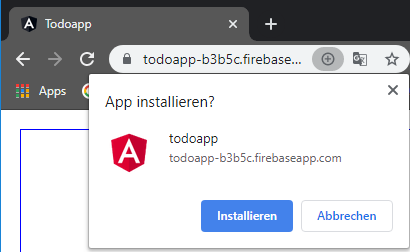
\includegraphics[width=0.48\textwidth]{img/add_to_desktop_2.PNG}
	\caption{Browser-Dialog zum Installieren der \ac{pwa} als Desktop-App}
	\label{fig:dialog_install_pwa_desktop}
\end{figure}

Damit dem Nutzer Benachrichtigungen tatsächlich angezeigt werden, muss er beim Erhalten der ersten Nachricht die Benachrichtigungen über einen Dialog aktivieren (s. Abb. \ref{fig:pwa_benachrichtigungen_zulassen}).
\begin{figure}[h!]	
	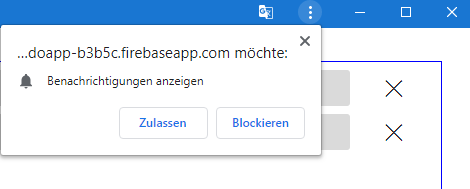
\includegraphics[width=0.48\textwidth]{img/berechtigungen_zulassen.PNG}
	\centering
	\caption{Browser-Dialog für Benachrichtigungen}
	\label{fig:pwa_benachrichtigungen_zulassen}
\end{figure}

\subsection{Aktualisieren der Anwendung}

Um das Update-Verhalten zu evaluieren, ist es interessant, den Update-Prozess einer Webanwendung bzw. einer \ac{pwa} zu betrachten. Um Änderungen an die Nutzer zu verteilen, muss ein Entwickler einen neuen \textit{Production Build} auf dem Server bereitstellen. Im Falle dieses Projekts werden Änderungen unter Nutzung des Firebase-\ac{cli} auf den Server übertragen.

In der Praxis werden die Änderungen in der installierten \ac{pwa} nicht sofort sichtbar, wohingegen die Webanwendung beim nächsten Refresh der Seite aktualisiert wird. Dies hängt mit dem Caching der Ressourcen der \ac{pwa} zusammen. Der Service Worker lädt cachebare Dateien entweder beim Start oder nachträglich, während die \ac{pwa} läuft, in den lokalen Cache des Geräts.

Um dieses Verhalten zu Testen, wurde ein Update mit einer auffälligen Hintergrundfarbe auf dem Server bereitgestellt. In der Desktop-\ac{pwa} war die Änderung erst nach einem System-Neustart zu sehen, wohingegen sich die \ac{pwa} unter Android nach einigen Stunden automatisch aktualisiert hatte. Dabei gab es jeweils keine Benachrichtigung zur Aktualisierung für den Nutzer.






